\documentclass{exam}

\usepackage{units} 
\usepackage[fleqn]{amsmath}
\usepackage{float}
\usepackage{mdwlist}
\usepackage{booktabs}
\usepackage{caption}
\usepackage{fullpage}
\usepackage{enumerate}
\usepackage{graphicx}
\usepackage{2in1, lscape} 

\everymath{\displaystyle}

\author{}
\date{January 22, 2014}
\title{Statistics \\ Course Overview}

\begin{document}

  \maketitle
  \section{Death Penalty Case Study}
  
  \subsection{Data}
  \begin{table}[ht]
  \centering
  \begin{tabular}{rlllr}
    \toprule
          & defendant & victim & sentence  & count \\
    \midrule
    1     & white & white & death     & 19 \\
    2     & white & black & death     & 0 \\
    3     & white & white & not death & 112 \\
    4     & white & black & not death & 9 \\
    5     & black & white & death     & 11 \\
    6     & black & black & death     & 6 \\
    7     & black & white & not death & 52 \\
    8     & black & black & not death & 97 \\
    \midrule
    total &       &       &           & 306 \\
    \bottomrule
  \end{tabular}
  \end{table}

  \subsection{By Sentence}

  12\% of the death penalty eligible cases with convictions resulted in death penalties.

  \begin{table}[H]
    \centering
    \begin{tabular}{lll}
      \toprule
      Death     & Not Death  & Total \\
      \midrule
      36 (12\%) & 270 (88\%) & 306 \\
       \bottomrule
    \end{tabular}
    \caption{Ignoring race}
  \end{table}

  \subsection{By Defendant Race}

  White defendants are more likely to get the death penalty than black defendants.

  \begin{table}[H]
    \centering
    \begin{tabular}{llll}
      \toprule
      Defendant & Death     & Not Death  & Total \\
      \midrule
      black     & 17 (10\%) & 149 (90\%) & 166 \\
      white     & 19 (14\%) & 121 (86\%) & 140 \\
      \bottomrule
    \end{tabular}
    \caption{By defendant race}
  \end{table}

  \subsection{By Defendant Race and Victim Race}

  For any race of victim, black defendants are more likely to get the death penalty than white defendants.

  \begin{table}[H]
    \centering
    \begin{tabular}{llll}
      \toprule
      Victim & Death     & Not Death & Total \\
      \midrule
      black  & 6 (6\%)   & 97 (94\%) & 103 \\
      white  & 11 (17\%) & 52 (83\%) & 63 \\
      \bottomrule
    \end{tabular}
    \caption{Black Defendant}
  \end{table}

  \begin{table}[H]
    \centering
    \begin{tabular}{llll}
      \toprule
      Victim & Death     & Not Death  & Total \\
      \midrule
      black  & 0 (0\%)   & 9 (100\%)  & 9 \\
      white  & 19 (15\%) & 112 (85\%) & 131 \\
      \bottomrule
    \end{tabular}
    \caption{White Defendant}
  \end{table}

  \subsection{By Victim}

  Cases with white victims are much more likely to result in the death penalty than cases with black victims.
  \begin{table}[H]
    \centering
    \begin{tabular}{llll}
      \toprule
      Victim & Death     & Not Death  & Total \\
      \midrule
      black  & 6 (5\%)   & 106 (95\%) & 112 \\
      white  & 30 (15\%) & 164 (85\%) & 194 \\
      \bottomrule
    \end{tabular}
  \end{table}

  \subsection{Summary}
  The race of the victim is an important factor in determining whether a case will result in the death penalty.  White
  defendants get the death penalty at a higher rate than black defendants because people tend to kill people of the same
  race.

  \begin{figure}[H]
    \centering
    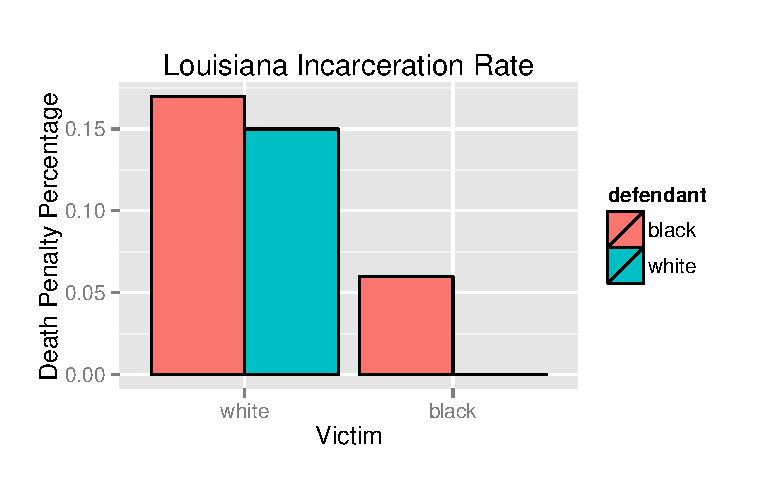
\includegraphics[scale = 0.9]{death_penalty.eps}
    \caption{Death Penalty Summary}
  \end{figure}

  \section{Course Areas}

  \subsection{Graphs}

  \subsection{Summary Statistics}

  \subsection{Sampling and Data Gathering}

\end{document}

